\section{Forward particle detector system}
A forward time of flight (TOF) counter system at 0 degrees with respect to the beam direction, which is installed to detect out-going neutrons and protons in the $^3$He($K^-$, $N$) reactions, is one of the most unique features in our spectrometer system. Flight lengths are kept more than 14 m for both neutrons and protons to achieve good momentum resolution, while keeping acceptance as much as $\sim$20 msr with a large volume of scintillator arrays. The forward TOF counter system is composed of a neutron counter array (NC), a proton counter array (PC) and a charged veto counter array (CVC) as illustrated in Fig. \ref{fig-forward}. The CVC located just upstream of the NC vetoes charged particles injected on the NC, not only detects fast protons. Trajectories of protons are reconstructed with a forward drift chamber 1 (FDC1) installed just downstream the target system, and bended by a dipole magnet named as Ushiwaka towards the PC. At the opposite side of the PC, we constructed a caved beam dump where kaon beams are swept out by Ushiwaka to suppress background events in the neutron spectrum. A beam veto counter (BVC), placed just downstream of the target cryostat, is used to reduce fake triggers for the neutral particle detection.

  \begin{figure}[]
   \begin{center}
    \includegraphics[width=0.9\columnwidth]{illustrator/forward.eps}
    \caption[Schematic view of the forward detectors]{Schematic view of the forward detectors;  the beam veto counter(BVC),  forward drift chamber 1 (FDC1), the beam sweeping magnet, the neutron counter (NC), the charge veto
    counter (CVC), and the proton counter (PC).
    The NC is located 14.7~m away from the final focus
    position.}
    \label{fig-forward}
   \end{center}
  \end{figure}  


\subsection{Neutron time-of-flight counter}
A neutron TOF counter (NC), located 14.7~m away from the final focus point, consists of an array of scintillation counters and has an effective volume of 3.2~m (horizontal) $\times$ 1.5~m (vertical) $\times$ 0.35~m (depth) segmented into 16-column (horizontal) $\times$ 7-layer (depth) units. The acceptance of the neutron counter is $\sim$ 20 msr ; $\pm$ 6.2$^\circ$ in the horizontal direction and $\pm$ 2.9$^\circ$ in the vertical. Each scintillation counter has dimensions of 20~cm (width) $\times$ 150~cm (height) $\times$ 5~cm (thickness) with two 2~inch Hamamatsu H6410 photomultipliers attached to both long sides of the scintillator through a Lucite light guide. The scintillators for the first three layers are made of Saint-Gobain BC408, and the other four layers are made of Saint-Gobain BC412. The average time resolution of the neutron counter, measured with cosmic
rays, is 92 $\pm$ 10~ps ($\sigma$). The error represents the variation among the segments.


\subsection{Charge veto counter}
The charge veto counter (CVC) is located upstream of the neutron counter, 14.0~m away from the final focus point and has an effective area of 3.4~m (horizontal)
$\times$ 1.5~m (vertical) segmented into 34 units. Each scintillation counter has dimensions of 10~cm (width) $\times$ 150~cm (height) $\times$ 3~cm (thickness), and is equipped with two 2~inch Hamamatsu H6410 photomultipliers attached to both long sides of the scintillator through a Lucite light guide. The scintillators are of Eljen EJ-200 type. The average time resolution measured with cosmic rays is 78 $\pm$ 7~ps ($\sigma$). The error represents the variation among the segments.


\subsection{Proton time-of-flight counter}
The proton TOF counter is installed as the extended wall of the charge veto counter. It has an effective area of 2.7~m (horizontal) $\times$ 1.5~m (vertical) segmented into 27 units.
The configuration of each scintillation counter is same with that of the charge veto counter except that a Saint-Gobain BC408 scintillator is used. The average time resolution of the proton counter, obtained from cosmic ray data, is 75 $\pm$ 6~ps ($\sigma$). The error represents the variation among the segments.


\subsection{Beam veto counter}
The beam veto counter (BVC) is attached on the downstream flange of the target cryostat as shown in Fig. \ref{fig:CDS}. The coverage size of the beam veto counter is 320~mm (height) $\times$ 320~mm (width) $\times$ 10~mm (thickness) made of Eljen EJ-200. This size is large enough to cover the acceptance of the neutron counter. The BVC is horizontally segmented into 8 units with different sizes as shown in Fig. \ref{fig-bvc} 
to avoid the over-concentration of the beam on the central segments. 1-inch fine-mesh Hamamatsu R5505 photomultipliers are attached on the both ends of each scintillator segment through Lucite light guides. The signals were read out with an amplification with HOSHIN preamplifier.

  \begin{figure}[]
   \begin{center}
    \includegraphics[width=\columnwidth]{illustrator/BVC.eps}
    \caption{Schematic drawing of the beam veto counter.}
    \label{fig-bvc}
   \end{center}
  \end{figure}  

\subsection{Forward drift chamber}
The forward drift chamber 1 (FDC1) is a feedthrough type chamber which has 6 planes with a VV'XX'UU' configuration. The tilt angles of $U$ and $V$ layers are $\pm$15 degrees. Each layer has 64 sense wires with a drift length of 3 mm which corresponds to an effective area of 384~mm (horizontal) $\times$ 264~mm (vertical). The cell geometry is shown in Fig \ref{fig-bldccell}(c) and the parameters of the chamber are summarized in Table \ref{tab-chamber}. 
The readout method is the same as those for the beam line chambers.

\if0
  \begin{figure}[]
   \begin{center}
    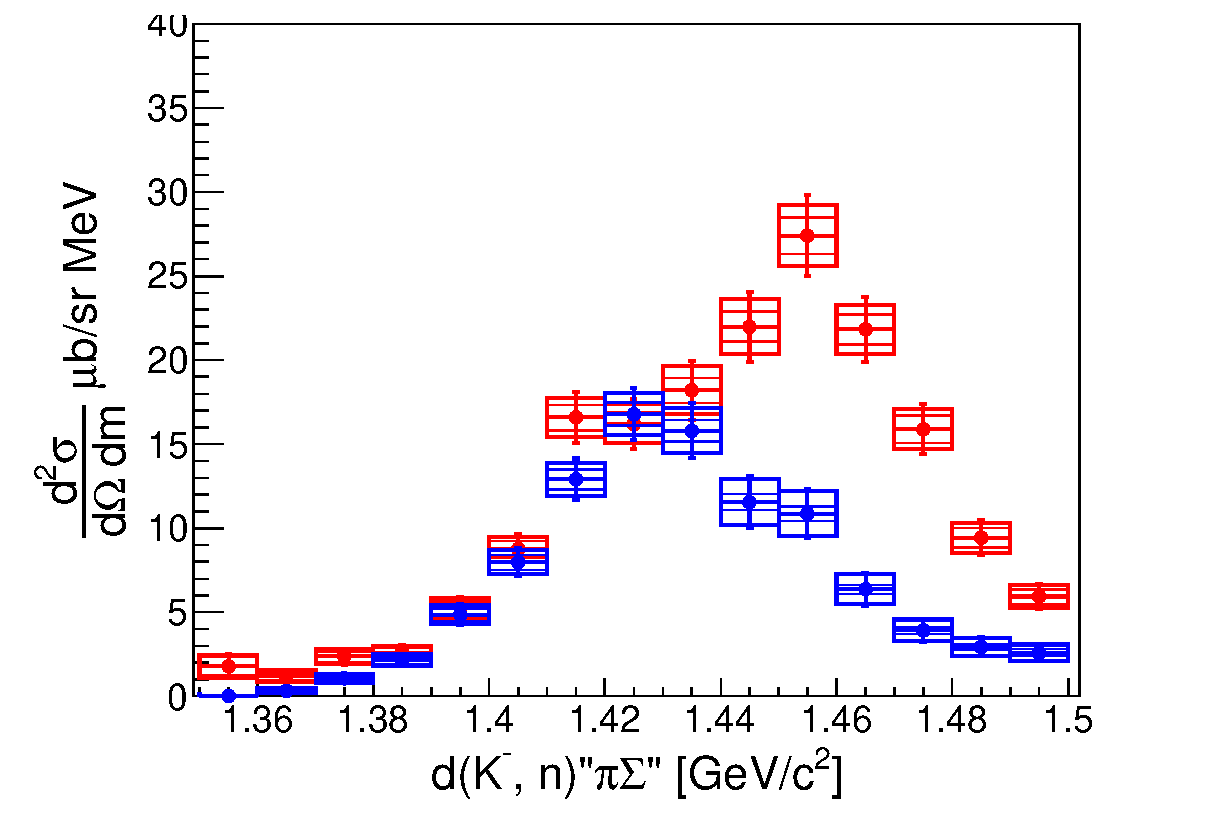
\includegraphics[width=10cm]{fig/tmp.eps}
    \caption{The cell structure of FDC1.}
    \label{fig-fdc1cell}
   \end{center}
  \end{figure}  
\fi

\subsection{Beam sweeping magnet}
A dipole magnet called Ushiwaka %, which was used in the $\pi$2 beam line of the 12 GeV proton synchrotron at KEK, is used as the beam sweeping magnet. It
is located downstream of the CDS and the FDC1 is attached on upstream of the magnet. The magnet has an aperture of 82~cm (horizontal) $\times$ 40~cm (vertical) and a pole length of 70~cm, which accommodates whole acceptance of the neutron counter. Ushiwaka is capable of providing a maximum field of 1.6 T and operated at $\sim$1.0 T in the production run. Figure \ref{fig-dumpprofile} shows the profile at the CVC and the PC with the inverse polarity setting of the Ushiwaka field. We confirmed that the central trajectory of the beam was well apart from the NC (CVC) acceptance, and the contamination in the NC acceptance was less than 3\%.  %Figure \ref{fig-uswkfield} shows a calculated magnetic field along beam axis, from which an effective pole length of 95 mm is obtained at the center of the aperture. 

 \begin{figure}[]
   \begin{center}
    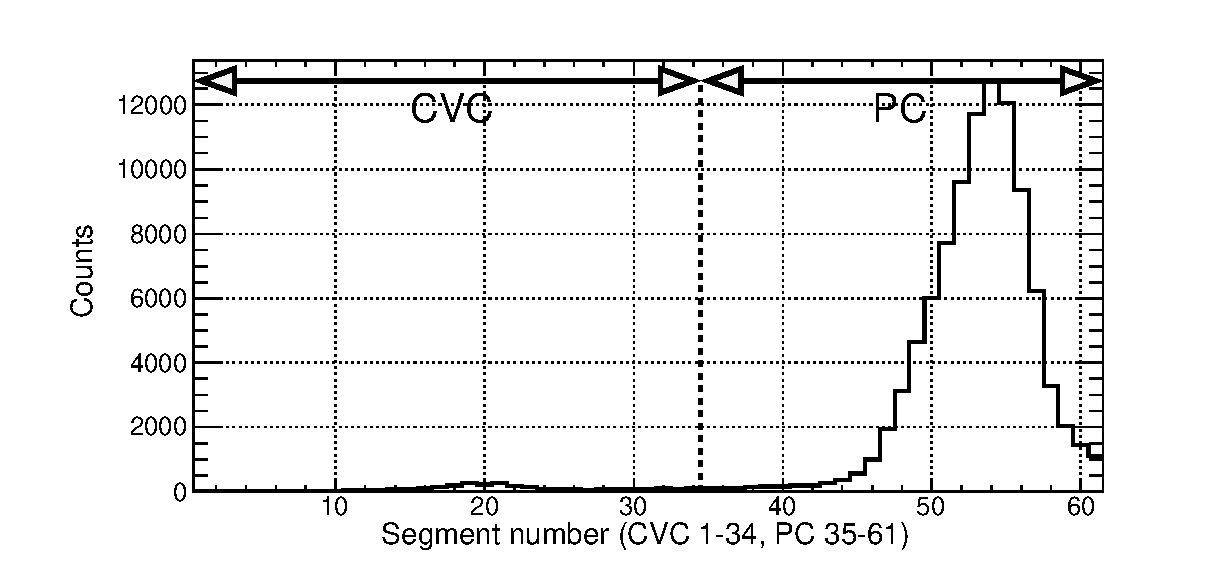
\includegraphics[width=0.9\columnwidth]{fig/dump.eps}
    \caption[Beam profile at the forward counters.]{Beam profile at the forward counters with the inverse polarity setting of the Ushiwaka field. Minimum biased beam data (BHD$\otimes$T0) is analyzed. The bump structure around CVC\#20 is mainly attributed to the pion charge exchange reaction, $\pi^-"p"\to\pi^0n,\ \pi^0\to 2\gamma$.}
    \label{fig-dumpprofile}
   \end{center}
  \end{figure}  

%  \begin{figure}[]
%   \begin{center}
%    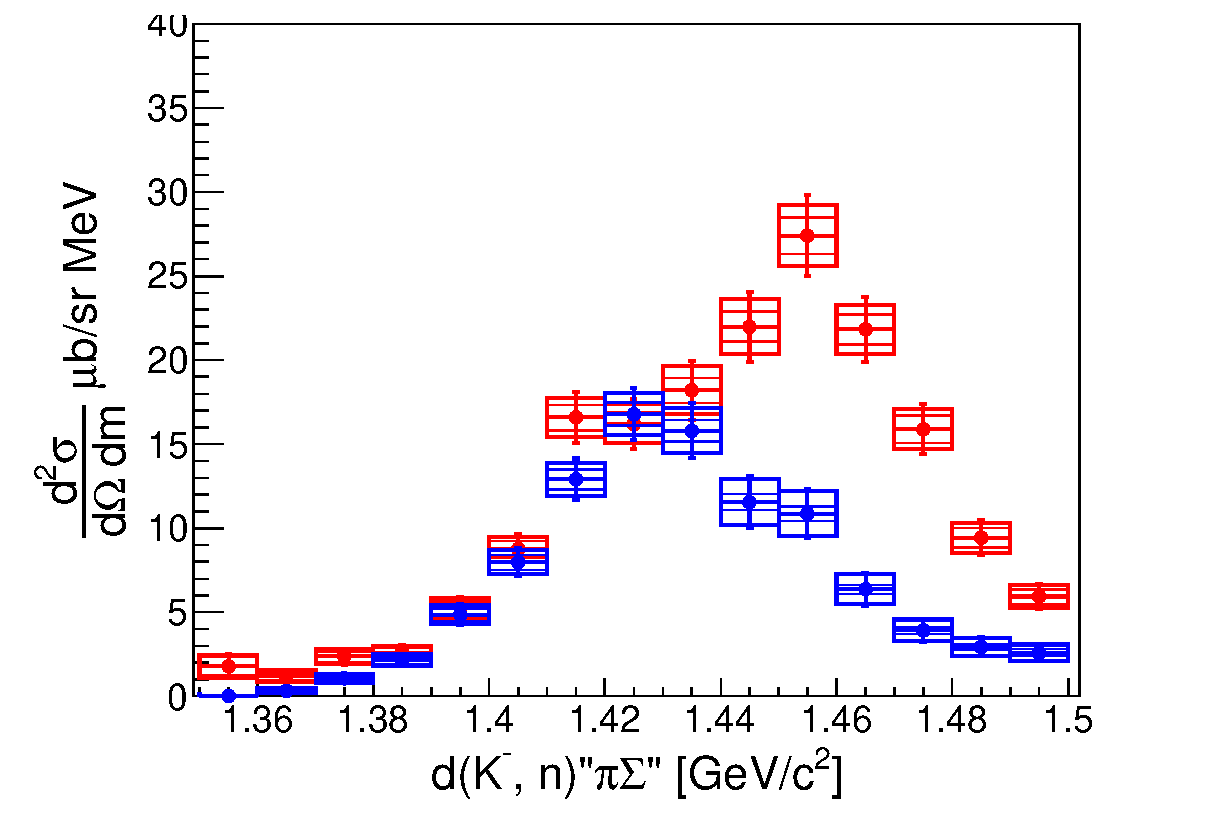
\includegraphics[width=10cm]{fig/tmp.eps}
%    \caption{A calculated field along Z (beam) axis of the Ushiwaka magnet .}
%    \label{fig-uswkfield}
%   \end{center}
%  \end{figure}  
